\documentclass{article}
\usepackage[utf8]{inputenc}
\usepackage{amsmath}
\usepackage{amssymb}
\usepackage{graphicx}
\usepackage{listings}

\lstdefinestyle{C++}
    {float=h!, frame=single, language={[Visual]C++}, numbers=left, numberstyle=\tiny, tabsize=2, breaklines=true}

\begin{document}
\section*{Kronecker product}
The Kronecker product is defined as follows.
\begin{figure}[!hbt]
    \centering
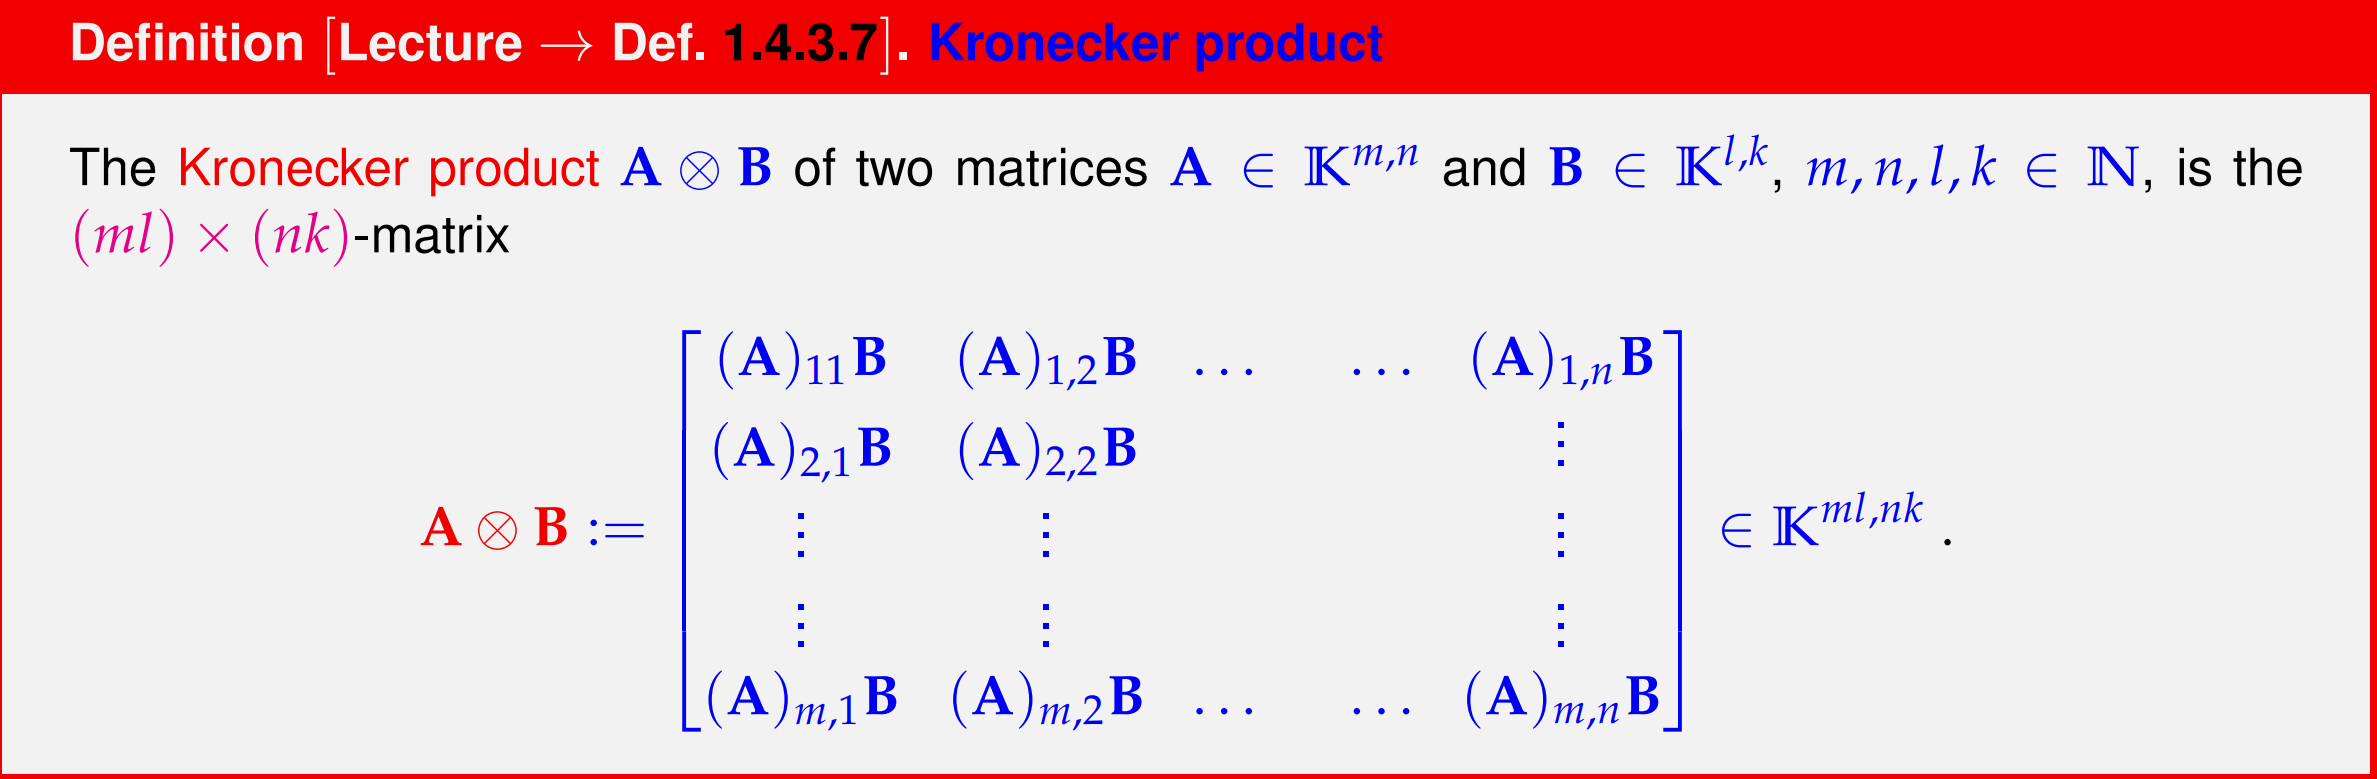
\includegraphics[width=1.0\linewidth]{KroeneckerProduct.png}
\end{figure}
\subsection*{1-3.a} We are given the matrices
\begin{equation*}
    \mathbf{A} = \begin{bmatrix}
        1 & 2 \\ 3 & 4
    \end{bmatrix} \qquad \mathbf{B} = \begin{bmatrix}
        5 & 6 \\ 7 & 8
    \end{bmatrix}
\end{equation*}
We should compute the Kronecker product of $\mathbf{A}$ and $\mathbf{B}$.
\begin{equation*}
    \mathbf{C} = \mathbf{A} \otimes \mathbf{B} = 
    \begin{bmatrix}
    \mathbf{A}_{1,1}\mathbf{B} & \mathbf{A}_{1,2}\mathbf{B} \\
    \mathbf{A}_{2,1}\mathbf{B} & \mathbf{A}_{2,2}\mathbf{B}
    \end{bmatrix} = 
    \begin{bmatrix}
    \mathbf{B} & 2\mathbf{B} \\
    3\mathbf{B} & 4\mathbf{B}
    \end{bmatrix} = 
    \begin{bmatrix}
     5 & 6 & 10 & 12 \\
     7 & 7 & 14 & 16 \\
     15 & 18 & 20 & 24 \\
     21 & 24 & 28 & 32
    \end{bmatrix}
\end{equation*}
\subsection*{1-3.b} We are tasked with implementing a \verb|C++| function that does the above computation. Luckily we can use the Eigen block operations to make out lives easier. We want to compute the following product

\begin{equation*}
    \mathbf{A} \otimes \mathbf{B} = \begin{bmatrix}
        \mathbf{A}_{1,1}\mathbf{B} & \mathbf{A}_{1,2}\mathbf{B} & \dots & \mathbf{A}_{1,n}\mathbf{B} \\
        \mathbf{A}_{2,1}\mathbf{B} & \mathbf{A}_{2,2}\mathbf{B} & \dots & \mathbf{A}_{2,n}\mathbf{B} \\
        \vdots & \vdots & & \vdots \\
        \mathbf{A}_{m,1}\mathbf{B} & \mathbf{A}_{m,2}\mathbf{B} & \dots &\mathbf{A}_{m,n}\mathbf{B} \\
    \end{bmatrix}
\end{equation*}

\pagebreak

This gives us the following code.
\begin{figure}[!hbt]
    \centering
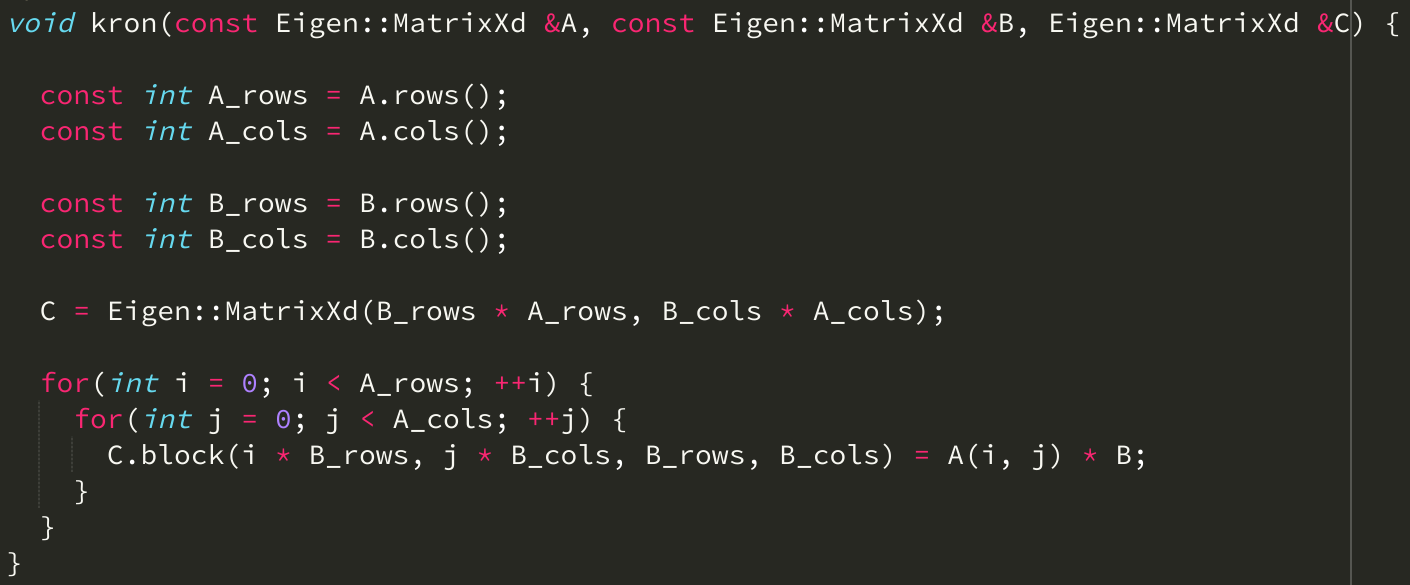
\includegraphics[width=1.0\linewidth]{1.3b.png}
\end{figure}
\subsection*{1-3.c} The asymptotic complexity is given by $n^{2}$ ($n \times n$ matrix)operations executed overall in the inner loop. The block operation in the inner loop multiplies a scalar with a a matrix, hence when passing a $n \times n$ matrix we get $\mathcal{O}\left(n^{2}\right)$ computational cost per inner loop body execution, thus totaling $\mathcal{O}\left(n^{2}\cdot n^{2}\right) = \mathcal{O}\left(n^{4}\right)$.
\subsection*{1-3.d} 
The computation of the entire matrix is unnecessary, we are now tasked with implementing an efficient implementation of the function \verb|kron_mult| which computes 
\begin{equation*}
    \mathbf{y} = \left(\mathbf{A} \otimes \mathbf{B}\right)\mathbf{x}
\end{equation*}
for square matrices $\mathbf{A}, \mathbf{B} \in \mathbb{R}^{n,n}$. $\\[1mm]$
Let us first look at the product, we have to check for compatibility in our code first, but here we assume the inputs are compatible. We have $\mathbf{A}\in \mathbb{K}^{m,n}$ and $\mathbf{B} \in \mathbb{K}^{l,k}$.
\begin{align*}
    \left(\mathbf{A}\otimes\mathbf{B}\right) &= \begin{bmatrix}
        \mathbf{A}_{1,1}\mathbf{B} & \mathbf{A}_{1,2}\mathbf{B} & \dots & \mathbf{A}_{1,n}\mathbf{B} \\
        \mathbf{A}_{2,1}\mathbf{B} & \mathbf{A}_{2,2}\mathbf{B} & \dots & \mathbf{A}_{2,n}\mathbf{B} \\
        \vdots & \vdots & & \vdots \\
        \mathbf{A}_{m,1}\mathbf{B} & \mathbf{A}_{m,2}\mathbf{B} & \dots & \mathbf{A}_{m,n}\mathbf{B} \\
    \end{bmatrix}
    \begin{bmatrix}
        x_{1:k} \\
        x_{k+1:2k} \\
        \vdots \\
        x_{\left(m-1\right)k +1:mk}
    \end{bmatrix}\\[2mm] &= 
    \begin{bmatrix}
        a_{11}\left(\mathbf{B}\cdot x_{1:k}\right) + a_{12}\left(\mathbf{B}\cdot x_{k+1:2k}\right) + \dots a_{1n}\left(\mathbf{B}\cdot x_{\left(m-1\right)k +1:mk}\right) \\
        a_{21}\left(\mathbf{B}\cdot x_{1:k}\right) + a_{22}\left(\mathbf{B}\cdot x_{k+1:2k}\right) + \dots a_{2n}\left(\mathbf{B}\cdot x_{\left(m-1\right)k+1:mk}\right) \\
        \vdots
        \\
        a_{m1}\left(\mathbf{B}\cdot x_{1:k}\right) + a_{m2}\left(\mathbf{B}\cdot x_{k+1:2k}\right) + \dots a_{mn}\left(\mathbf{B}\cdot x_{\left(m-1\right)k +1:mk}\right)
        \end{bmatrix}
\end{align*} 

\pagebreak

\noindent We can now see that this repeats the same operation over and over again, hence we would rather compute the following matrix-vector-like product instead.
\begin{equation*}
    \begin{bmatrix}
        a_{11} & a_{12} & \dots & a_{1n} \\
        a_{21} & a_{22} & \dots & a_{2n} \\
        \vdots & \vdots & & \vdots \\
        a_{m1} & a_{m2} & \dots & a_{mn} \\
    \end{bmatrix}
    \odot
    \begin{bmatrix}
        \mathbf{B}\cdot x_{1:l} \\
        \mathbf{B}\cdot x_{l+1:2l} \\
        \vdots \\
        \mathbf{B}\cdot x_{\left(m-1\right)l +1:ml}
    \end{bmatrix}
\end{equation*}
This results in the following code.
\begin{figure}[!hbt]
    \centering
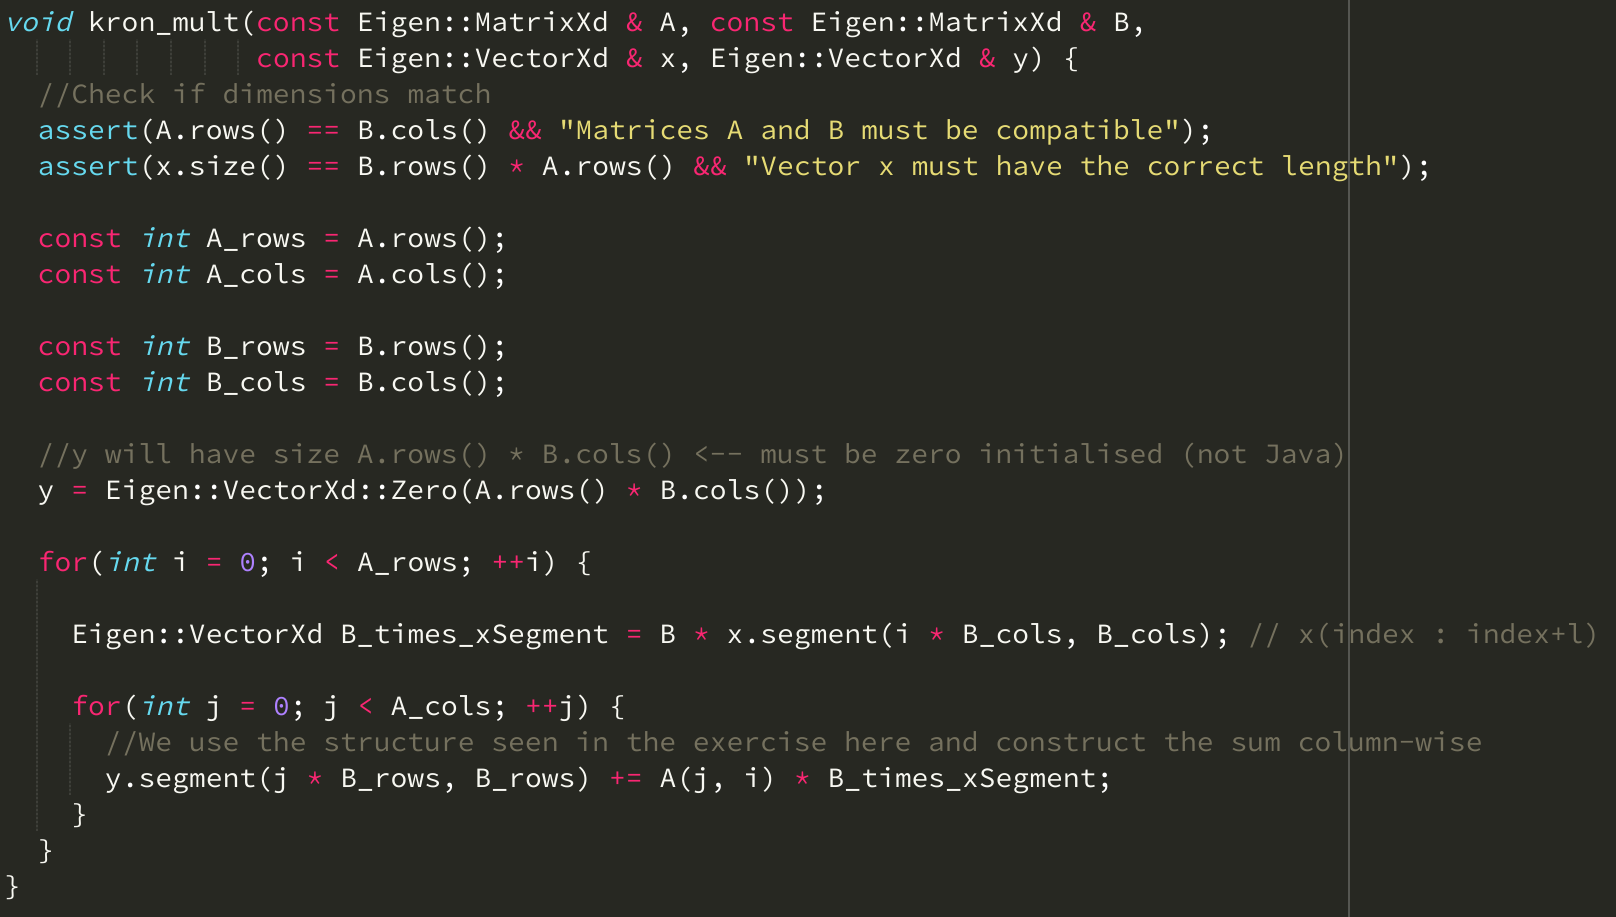
\includegraphics[width=1.2\linewidth]{1-3c.png}
\end{figure}
The code was only tested for square matrices, so there may be some index mismatches in there.
\subsection*{1-3.e}
We are now tasked with using the reshape operation of Eigen instead of the segment function. We will write this method assuming the inputs are square matrices for simplicity. Let us look at a $2\times 2$ example to understand how this would work.
\begin{equation*}
    \left(\begin{bmatrix}
        a_{11} & a_{12} \\
        a_{21} & a_{22}
    \end{bmatrix}
    \otimes
    \begin{bmatrix}
        b_{11} & b_{12} \\
        b_{21} & b_{22}
    \end{bmatrix}\right)
    \begin{bmatrix}
        x_{1} \\x_{2} \\x_{3} \\x_{4}
    \end{bmatrix} = \begin{bmatrix}
    a_{11}b_{11} & a_{11}b_{12} & a_{12}b_{11} & a_{12}b_{12} \\
    a_{11}b_{21} & a_{11}b_{22} & a_{12}b_{21} & a_{12}b_{22} \\
    a_{21}b_{11} & a_{21}b_{12} & a_{22}b_{11} & a_{22}b_{12} \\
    a_{21}b_{21} & a_{21}b_{22} & a_{22}b_{21} & a_{22}b_{22} 
\end{bmatrix}\begin{bmatrix}
        x_{1} \\x_{2} \\x_{3} \\x_{4}
    \end{bmatrix}
\end{equation*} 

\pagebreak

\noindent Which then gives us
\begin{equation*}
    \begin{bmatrix}
    a_{11}b_{11} & a_{11}b_{12} & a_{12}b_{11} & a_{12}b_{12} \\
    a_{11}b_{21} & a_{11}b_{22} & a_{12}b_{21} & a_{12}b_{22} \\
    a_{21}b_{11} & a_{21}b_{12} & a_{22}b_{11} & a_{22}b_{12} \\
    a_{21}b_{21} & a_{21}b_{22} & a_{22}b_{21} & a_{22}b_{22} 
\end{bmatrix}\begin{bmatrix}
        x_{1} \\x_{2} \\x_{3} \\x_{4}
    \end{bmatrix} = \begin{bmatrix}
         a_{11}b_{11}x_{1} + a_{11}b_{12}x_{2} + a_{12}b_{11}x_{3} + a_{12}b_{12}x_{4} \\
         a_{11}b_{21}x_{1} + a_{11}b_{22}x_{2} + a_{12}b_{21}x_{3} + a_{12}b_{22}x_{4} \\
         a_{21}b_{11}x_{1} + a_{21}b_{12}x_{2} + a_{22}b_{11}x_{3} + a_{22}b_{12}x_{4} \\
         a_{21}b_{21}x_{1} + a_{21}b_{22}x_{2} + a_{22}b_{21}x_{3} + a_{22}b_{22}x_{4}
    \end{bmatrix}
\end{equation*}
Let us look at the following square reshape of $\mathbf{x}$ (EIGEN maps fill columns first)
\begin{equation*}
    \begin{bmatrix}
        x_{1} \\ x_{2} \\x_{3} \\x_{4}
    \end{bmatrix}
    \mapsto
    \begin{bmatrix}
        x_{1} & x_{3} \\
        x_{2} & x_{4}
    \end{bmatrix}
\end{equation*}
We can then look at the following product
\begin{equation*}
    \begin{bmatrix}
        b_{11} & b_{12} \\
        b_{21} & b_{22}
    \end{bmatrix}
    \begin{bmatrix}
        x_{1} & x_{3} \\
        x_{2} & x_{4}
    \end{bmatrix}
    = 
    \begin{bmatrix}
    b_{11}x_{1} + b_{12}x_{3} & b_{11}x_{2} + b_{12}x_{4} \\
    b_{21}x_{1} + b_{22}x_{3} & b_{21}x_{2} + b_{22}x_{4}
    \end{bmatrix}
\end{equation*}
One can spot how this pattern nicely lines up with the above matrix vector product. How do we now add $\mathbf{A}$ to this result to produce the desired result? We can see that the result would be a matrix, as we do a matrix-matrix multiplication, hence we would probably require another reshape. We could reshape this matrix to get the result we want.
\begin{equation*}
    \begin{bmatrix}
         a_{11}b_{11}x_{1} + a_{11}b_{12}x_{2} + a_{12}b_{11}x_{3} + a_{12}b_{12}x_{4} &
         a_{11}b_{21}x_{1} + a_{11}b_{22}x_{2} + a_{12}b_{21}x_{3} + a_{12}b_{22}x_{4} \\
         a_{21}b_{11}x_{1} + a_{21}b_{12}x_{2} + a_{22}b_{11}x_{3} + a_{22}b_{12}x_{4} &
         a_{21}b_{21}x_{1} + a_{21}b_{22}x_{2} + a_{22}b_{21}x_{3} + a_{22}b_{22}x_{4}
    \end{bmatrix}
\end{equation*}
This, as one can quickly verify, is the result of the following matrix-matrix multiplication.
\begin{align*}
    \begin{bmatrix}
    b_{11}x_{1} + b_{12}x_{3} & b_{11}x_{2} + b_{12}x_{4} \\
    b_{21}x_{1} + b_{22}x_{3} & b_{21}x_{2} + b_{22}x_{4}
    \end{bmatrix}\begin{bmatrix}
    a_{11} & a_{21} \\
    a_{12} & a_{22}
    \end{bmatrix} 
    = 
\underbrace{
    \begin{bmatrix}
        b_{11} & b_{12} \\
        b_{21} & b_{22}
    \end{bmatrix}}_{\mathbf{B}} \underbrace{
    \begin{bmatrix}
        x_{1} & x_{3} \\
        x_{2} & x_{4}
\end{bmatrix}}_{\text{reshaped } \mathbf{x}} \underbrace{\begin{bmatrix}
    a_{11} & a_{21} \\
    a_{12} & a_{22}
\end{bmatrix}}_{=\mathbf{A}^{\mathsf{T}}}
\end{align*}

\noindent We have
\begin{align*}
    &\begin{bmatrix}
        b_{11} & b_{12} \\
        b_{21} & b_{22}
    \end{bmatrix}
    \begin{bmatrix}
        x_{1} & x_{3} \\
        x_{2} & x_{4}
\end{bmatrix}
\begin{bmatrix}
    a_{11} & a_{21} \\
    a_{12} & a_{22}
\end{bmatrix} = \begin{bmatrix}
    b_{11}x_{1} + b_{12}x_{2} & b_{11}x_{3} + b_{12}x_{4} \\
    b_{21}x_{1} + b_{22}x_{2} & b_{21}x_{3} + b_{22}x_{4}
\end{bmatrix}\begin{bmatrix}
    a_{11} & a_{21} \\
    a_{12} & a_{22}
\end{bmatrix} \\
&= \begin{bmatrix}
    \left(a_{11}b_{11}x_{1} + a_{12}b_{11}x_{1}\right) + \left(a_{11}b_{12}x_{2} + a_{12}b_{12}x_{2}\right) & \left(a_{21}b_{11}x_{3} + a_{22}b_{11}x_{3}\right) + \left(a_{21}b_{12}x_{4} + a_{22}b_{12}x_{4}\right) \\
    \left(a_{11}b_{21}x_{1} + a_{12}b_{21}x_{1}\right) + \left(a_{11}b_{22}x_{2} + a_{12}b_{22}x_{2}\right) + \left(a_{11}b_{22}x_{2} + a_{12}b_{22}x_{2}\right) & \left(a_{21}b_{21}x_{3} + a_{22}b_{21}x_{3}\right) + \left(a_{21}b_{22}x_{4} + a_{22}b_{22}x_{4}\right)
\end{bmatrix}
\end{align*}
From here we do one more reshape and we get our result. Reshaping in EIGEN uses the following syntax $\\[2mm]$
\verb|Eigen::MatrixXd::Map(x.data(), n, n);| $\\[1mm]$
This reshapes the data of $\mathbf{x}$ which means a contiguous arrangement of elements into a $n \times n$ structure, while filling up the structure \textbf{column-major}, hence filling the columns first, if the dimensions are larger than the amount of elements in \verb|x.data()| then whatever was in the memory locations before will be the new entries of the mapped to structure. Reshaping to smaller dimensions does not work and will give an assertion error.

\pagebreak

\noindent The following code results from this.

\begin{figure}[!hbt]
    \centering
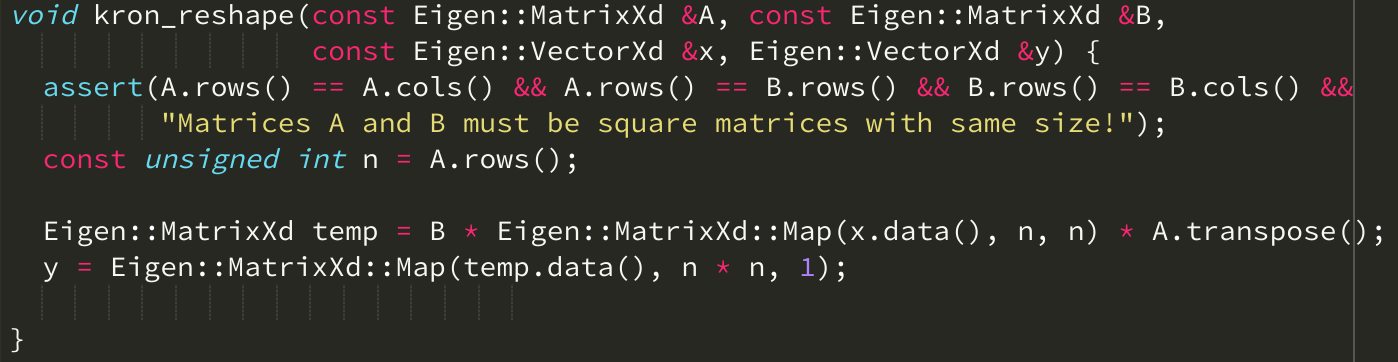
\includegraphics[width=1.2\linewidth]{1-3d.png}
\end{figure}
\subsection*{1-3.f}
We again skip this section as it brings little to no value.

\end{document}
